\chapter{Les devis\index{Devis}}
Les devis représentent l'une des fonctionnalités principales de l'application. Il est possible de créer plusieurs devis pour un seul projet d'un client. 
\section{Liste des devis\index{Devis!Liste}}
Pour afficher les devis d'un projet il faut, à partir du panneau contenant la liste des projets d'un client, faire un double clic sur le projet en question. La liste affichée contient les factures et les devis du projet sélectionné auparavant.
\begin{figure}[H]
	\centering
	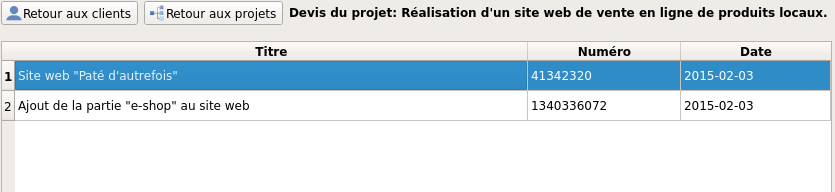
\includegraphics[width=12cm]{screens/ihmDevis.png}
	\caption{Liste des devis et factures d'un projet}
\end{figure}
Les devis apparaissant dans la liste peuvent être ouvert au format PDF. Il suffit de sélectionner le devis dans la liste puis de cliquer sur le bouton << Ouvrir le PDF >>. 
\begin{figure}[H]
	\centering
	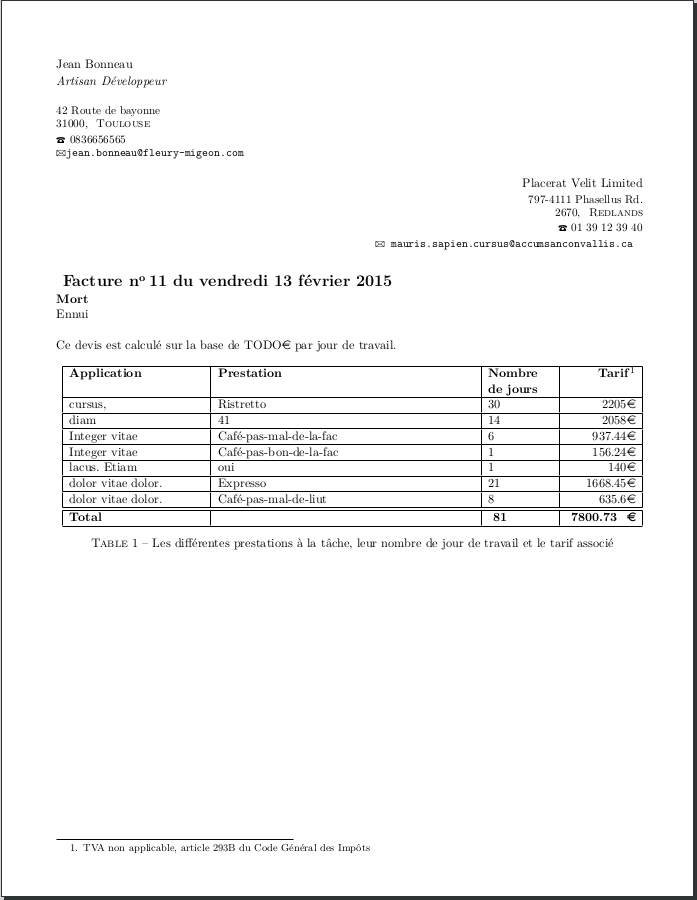
\includegraphics[width=7cm]{screens/genererPDF.png}
	\caption{Ouvrir un devis au format PDF}
	\label{fig:ouvrirPDF}
\end{figure}
\section{Ajouter un devis\index{Devis!Ajouter}}
\label{ch:ajoutDevis}
Pour ajouter un devis, il est nécessaire de sélectionner un client dans le panneau central (si l'on est dans la liste des projets ou des devis, le nouveau devis sera automatiquement ajouté à ce client). Une fois le client sélectionné on crée un nouveau devis en cliquant sur le bouton << Nouveau devis >> de la barre d'outils ou via le menu << Client $\rightarrow$ Nouveau devis >>. 
\begin{figure}[H]
	\centering
	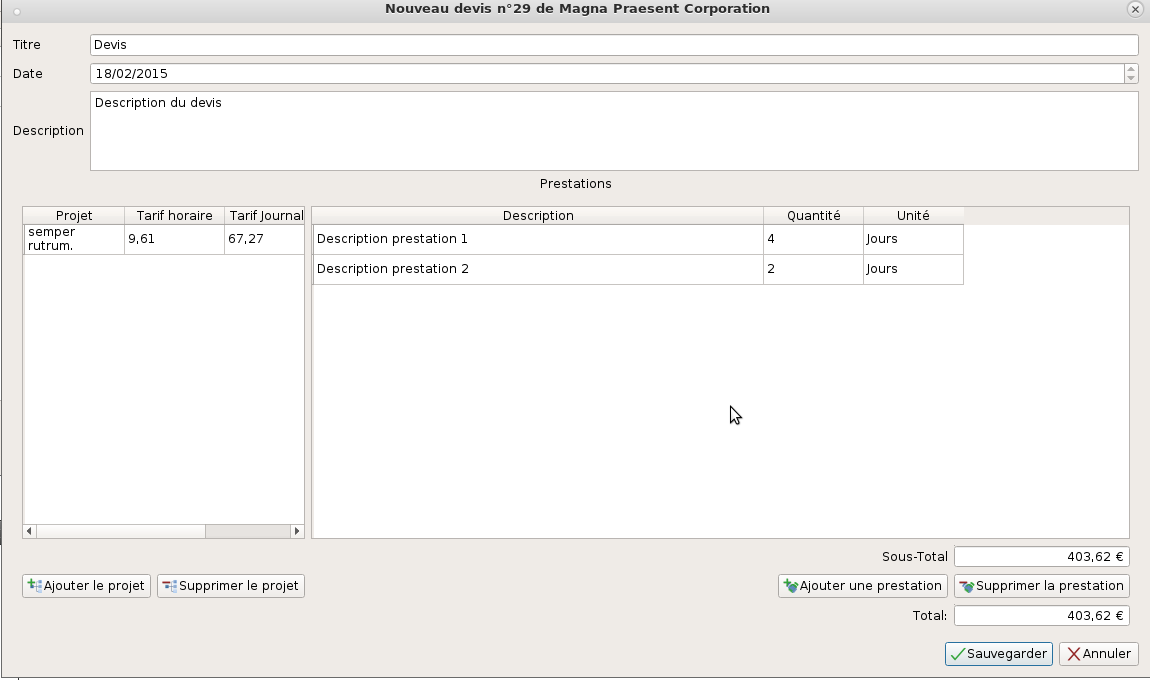
\includegraphics[width=17cm]{screens/creerDevis.png}
	\caption{Créer un nouveau devis pour un projet client}
	\label{fig:creerDevis}
\end{figure}
Un devis possède un titre à afficher, une date (celle du jour de création du projet) et une description. Plus bas arrivent deux tableaux: celui de gauche correspond aux différents projets appelés dans le devis avec pour chacun, le tarif horaire et le tarif journalier qui sont à déterminer. En sachant que modifier l'un va entraîner la modification de l'autre et vice-versa. Le tableau de droite, qui n'apparaît pas au lancement de la fenêtre représente les prestations d'un projet. Tout les prix affichés, que cela soit le sous-total (total d'un projet) ou le total de tous les projets, tous sont calculés automatiquement en fonction du tarif horaire et journalier défini pour le projet et de la quantité de temps définie pour une prestation.

Il est également possible de créer un nouveau devis à partir d'un existant via le bouton << copier le devis >>. Après ouverture de la fenêtre contenant les informations du modèle, il est possible de changer le nouveau devis en facture. 
\section{Editer un devis\index{Devis!Editer}}
Pour éditer un devis, il faut nécessairement cliquer dessus sur le tableau affichant les devis et les factures d'un projet. Une fois le devis sélectionné, on affiche la fenêtre d'édition de devis en cliquant sur le bouton << Editer le devis >> en dessous du tableau.
La fenêtre qui s'affiche est en tout point semblable à la fenêtre d'ajout d'un devis \ref{fig:creerDevis} hormis le fait que tous les champs sont déjà pré-remplis.

\section{Les Prestations\index{Devis!Prestation}}
\label{ch:Prestations}
La liste des prestations s'affiche dans la fenêtre d'ajout d'un devis\index{Devis!Ajouter} lorsqu'il y a au moins un projet défini dans le tableau des projets et que celui-ci est sélectionné. Une prestation peut être ajoutée, respectivement supprimée en utilisant les boutons << Ajouter une prestation >> et << Supprimer la prestation >>. Dans le cas d'un ajout, une nouvelle ligne est ajoutée au tableau des prestations. Cette ligne indique une description de la prestation et le nombre et la quantité de temps qui va y être consacrée. L'unité de temps est modifiable avec le choix entre jours et heures.

